<<<<<<< HEAD
\documentclass[a4paper ]{report}
=======
\documentclass{report}
>>>>>>> master
% 导言区
\usepackage{xeCJK}
\usepackage{graphicx}
\graphicspath{{figures/}}
\usepackage{float}
\usepackage{amsmath}
% 加深编号
\setcounter{secnumdepth}{3}
% 标题信息
\title{移动通信}
\author{张兴锐}
\date{2018-3-25}
\begin{document}
	\maketitle
	\tableofcontents
	% 
<<<<<<< HEAD
		\chapter{概论}
	\section{移动通信特点}
	\subsection{什么是移动通信?}
	\textbf{定义:}移动通信就是通信双方至少有一方是处于运动中进行信息交换的通信方式。其移动性包括:
	\begin{itemize}
		\item 终端的移动性,特定的“终端号码(如手机串号,\verb|*#06#| )“,手机,车载台
		\item 个人的移动性,特定的”个人号码,SIM卡号”。
	\end{itemize}
	\subsection{移动通信特点}
	\begin{enumerate}
		\item 移动通信必须利用无线电波进行信息传输。
		\begin{enumerate}
			\item 弥散损耗(自由传播损耗),随着传播距离的增加而损耗。
			\item 阴影效应,受到地形、地物的遮蔽而发生。
			\item 多径效应,信号经过多点反射,会从多条路径到达接受地点,这种多径信号的\textbf{幅度、相位和到达时间}都不一样,它们会叠加而产生“多径效应”。
			\item 多普勒-效应
		\end{enumerate}
		\item 移动通信是在复杂的干扰环境中运行的。
		\begin{enumerate}
			\item 外部干扰。天电干扰、工业干扰和信道噪声
			
			\item 系统间干扰。
			\begin{enumerate}
				\item 邻道干扰
				\item 互调干扰(当两个或多个干扰信号同时加到接收机时,\textbf{由于非线性的作用},这两个干扰的组合频率有时会恰好等于或接近有用信号频率而顺利通过接收机,这种干扰就称为互调干扰,其中三阶互调最严重。)
				\item 同频道
				干扰(蜂窝移动通信)
				\item 多址干扰(多址干扰是指同\textbf{CDMA}系统中多个用户的信号在时域和频域上是混叠的。因为\textbf{CDMA}系统为码分多址,CDMA系统采用的是不同的地址码来区分每个用户,但多个用户的信号在时域和频域上是混叠的,所以在频域在产生一定的同频和邻频干扰,则为多址干扰。)
				\item 远近效应
			\end{enumerate}
			
			\item 抗干扰技术。扩频技术、信道编码与交织技
			术、信道均衡技术、分集技术、信道估计技
			术、信号检测技术和智能天线技术
			
		\end{enumerate}
		\item 移动通信业务量的需求与日俱增,而频率资源
		非常有限。
		\item 移动通信系统的网络结构多种多样,网络管
		理和控制必须有效。
		\item 移动通信设备必须适于在移动环境中满足多种应
		用要求。
	\end{enumerate}
	\section{常用移动通信系统}
	\begin{enumerate}
		\item 蜂窝移动通信系统
		\item  公共陆地移动通信网络(PLMN)
		\item 无线市话系统(WUTS)
		\item 集群系统(专网)--->公安系统,水利系统、交通系统、电力系统、铁路系统。
		\item 卫星移动通信系统。
		\item 无线局域网。
	\end{enumerate}
	\section{移动通信系统发展}
	\subsection{各代通信系统特点}
	\begin{description}
		\item[第一代] 模拟,仅限语音,仅限宏小区
		\item[第二代]  数字,语音和数据通信,宏/微小区
		\item[第三代] 频谱利用率高,传输速率按需分配
		\item[第四代] 更高的数据速率和更大的系统容量,正交频分复用(OFDM)技术、
	\end{description}
	\begin{figure}[H]
		\centering
		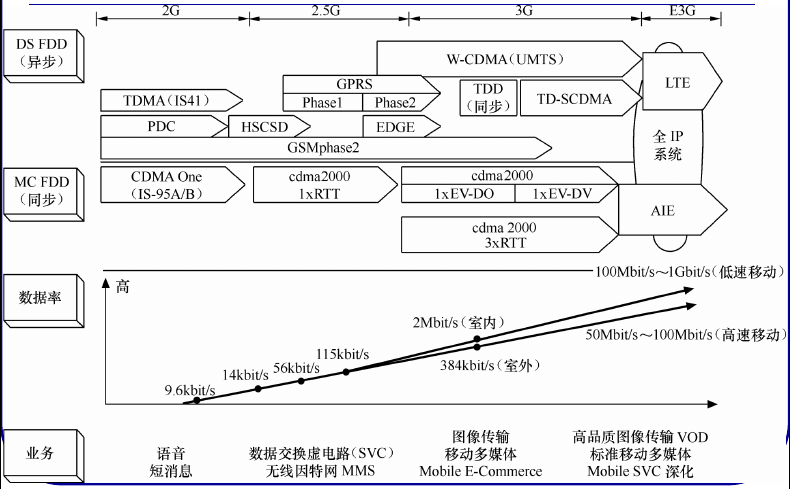
\includegraphics[scale=0.7]{移动通信系统2G_4G发展.png}
		\caption{移动通信系统发展}
	\end{figure}
	\begin{figure}[H]
		\centering
		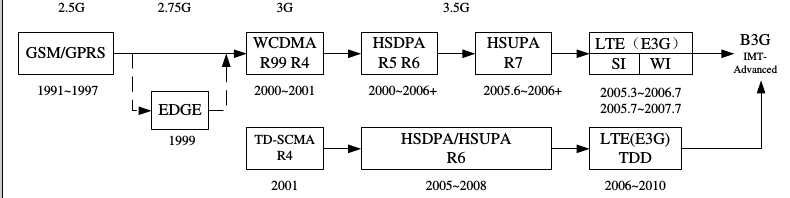
\includegraphics[scale=0.7]{WCDMA_TD-SCDMA发展.png}
		\caption{WCDMA\&TD-SCDMA发展}
	\end{figure}
	\begin{figure}[H]
		\centering
		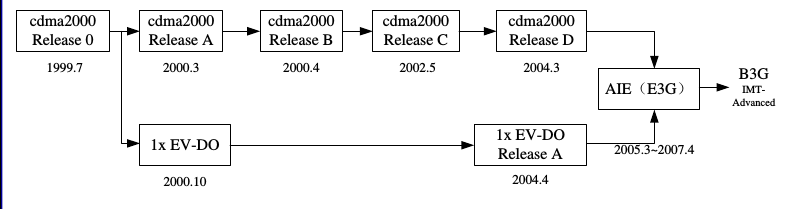
\includegraphics[scale=0.7]{CDMA2000发展.png}
		\caption{CDMA2000发展}
	\end{figure}
	
	\section{移动通信基本技术}
		\begin{figure}[H]
			\centering
			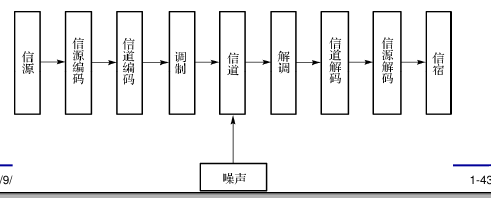
\includegraphics[scale=1]{信号传输过程.png}
			\caption{信号传输过程}
		\end{figure}
	\begin{description}
		\item[信源编码技术
		] 以提高通信有效性为目的而对信源符号进
		行的变换。
		\begin{enumerate}
			\item 波形编码
			\item 参数编码
			\item 混合编码
		\end{enumerate}
		\item[信道编码技术
		] 为了减少差错,信道编码器对传输的信息码
		元按一定的规则加入保护成分(监督元),
		组成所谓“抗干扰编码”;
		提高通信系统抗干扰能力,实现可靠通信。\\分组码、卷积码。
		\item[调制技术
		] 使要传输的信息适合于信道特征,
		达到有效、可靠的传输 。\\连续相位调制,线性调制,PSK,QPSK,DQPSK,QAM等。
		\item[电波传播特性的研究
		]  总结和建立有普遍性的数学模型,利用这些
		模型,可以估算一些传播环境中的传播损耗
		和其它有关的传播参数。
	\end{description}
	\section{蜂窝移动通信的组网技术}
	\subsection{多址接入}
	\subsubsection{什么是多址接入?}
	\textbf{定义:}移动通信系统中,使所有的用户共享
	有限的无线资源,实现不同用户不同地点同时
	通信,并尽可能减少干扰。
	\subsubsection{多路复用和多址接入区别}
	\textbf{相同点:}两者的理论基础都是\textbf{信号的正交分割原理。}\\
	\textbf{不同点:}
	\begin{itemize}
		\item \textbf{”点对点“},多路复用
		\item \textbf{"点多多点"},多址接入
	\end{itemize}
	
	\subsubsection{多址接入分类}
	\begin{enumerate}
		\item 频分多址: 第一代移动通信系统;TACS、AMPS。\\特点:
		\begin{itemize}
			\item 一个频道传送一路电话,一旦给用户分配频道,移动台和基站同时连续不断发射
			\item 信道带宽较窄。
			\item 传输速率地,码元持续时间长,与平均延迟扩展相比很大,\textbf{码间干扰不需要均衡}
			\item 系统简单,但需要一个双工器,同事需要一个RF(射频)滤波器。
		\end{itemize}
		展造成的符号间干扰低。
		\item 时分多址: 第二代移动通信系统:GSM。\\特点:
		\begin{itemize}
			\item 多个用户共享一个载波频率,分享不同时隙。
			\item 分组可以实现不连续发送。
			\item {\color{red}{由于速率较高,往往需要均衡器。}}
			\item 需要额外开销,如保护时隙,\textbf{同步}时隙等。
			\item 按照不同用户提供不同的带宽。
		\end{itemize}
		\item 码分多址: 第三代移动通信系统:IS-95 CDMA、WCDMA。\\特点:
		\begin{itemize}
			\item 通过不同的码序列来划分物理信道,信道在时间
			和频率上重合
			\item 码不但可以区分信道(walsh和OVSF),还可以区分基站(gold)或用户(m序列)
			\item  CDMA系统的许多用户共享同一频率
			\item 由于信号被扩展在一较宽频谱上,所以可\textbf{减小多
			径衰落;}
			\item 在CDMA系统中,信道数据速率很高,采用分集
			接收最大比合并技术,可获得最佳的抗多径衰落
			效果;
			\item 软切换和有效的宏分集
			\item  低信号功率谱密度
		\end{itemize}
		存在两个重要问题:
		\begin{enumerate}
			\item  多址干扰
			\item  远近效应.
		\end{enumerate}
		\item 空分多址。特点:
		\begin{itemize}
			\item 实现空间分割的基本技术就是\textbf{自适应阵列天线},在不同的用户方向上形成不同的波束。
			\item 有效地克服\textbf{多径干扰和同频道干扰}
		\end{itemize}
		\item OFDMA.正交频分多址接入
		\item NOMA,非正交频分多址接入
	\end{enumerate}
	\subsection{工作方式}
	\begin{enumerate}
		\item 单工::通信双方电台交替地进行收信和
		发信。\textbf{对讲机}。
		\item 半双工:是指通信双方中,一方使用双
		频双工方式,即收发信机同时工作;另一
		方使用双频单工方式,即收发信机交替工
		作。\textbf{基站-手机}。基站处于全双工,手机处于半双工。
		\item 全双工:是指通信双方收发信机均同时工作。收信和发信必须\textbf{采用不同的工作频率},\textbf{打电话}	\\
		双工模式:
		\begin{enumerate}
		\item 频分双工FDD:通信双方收发信可同时进行,但收信和发信分别占用两个不同的频率。
		\item 时分双工TDD:使用相同频率,但不同的时隙进行区分。
		\end{enumerate}
		两种模式的区别:
		
		\begin{itemize}
			\item TDD可灵活配置频率,\textbf{使用FDD系统不易使用的零散
			频段};但为避免与其他无线系统之间的干扰,TDD
			需预留较大的保护带,影响\textbf{整体频谱利用效率}。
			\item TDD可以通过调整上下行时隙转换点,改变上下行
			时隙比例,可\textbf{很好地支持非对称业务}。
			TDD系统\textbf{收发信道同}频,无法进行干扰隔离,速度
			越快,衰落变换频率越高,衰落深度越深;相当于
			混合行驶,容易撞车,因此必须要求\textbf{移动速度不能
			太高}。
			\item TDD接收上/下行数据时,不需收发隔离器,只需一
			个开关即可,降低设备的复
			\item 由于TDD方式的时间资源\textbf{分别分给了上行和下行,
			因此TDD方式的发射时间大约只有FDD的一半},如果
			TDD要发送和FDD同样多的数据,就要\textbf{增大TDD的发
			送功率}
			\item TDD系统上行受限,因此TDD基站的\textbf{覆盖范围明显小}
			于FDD基站。
			\item FDD模式的特点是在分离(上下行频率间隔45MHz
			190MHz等)的两个对称频率信道上,系统进行接收
			和传送,用保护频段来分离接收和传送信道。相当
			于分道行驶,比较顺畅,所以\textbf{FDD速度会更快}。
		\end{itemize}
	
		\begin{center}
			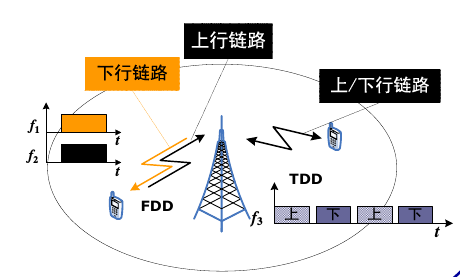
\includegraphics[scale=1]{双工模式.png}
		\end{center}
	\end{enumerate}
	\subsection{频率复用和蜂窝小区}
	\subsubsection{移动通信网的区域覆盖方式}
	\begin{enumerate}
		\item 小容量的大区制(发射功率大),基站发射功率要大,利用分集接收等技术来保证上行链路的通信质量。
		\item  大容量的小区制,(频率复用),同频干扰问题
	\end{enumerate}
	\subsubsection{区群}
	\begin{minipage}{0.4\linewidth}
	\textit{要想正多边形无空隙、无重叠地覆盖一个平面的区域,只有\textbf{正三角形、正方形和正六边形三种形状}}
	\end{minipage}
	\begin{minipage}{0.4\linewidth}
		\centering
		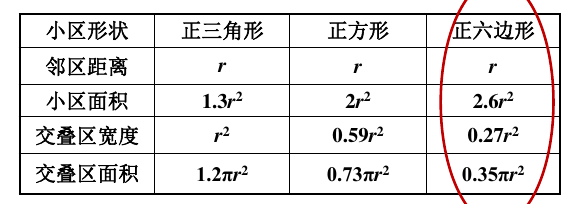
\includegraphics[scale=0.6]{三种形状方案.png}
	\end{minipage}\\
	 \textbf{定义:}共同使用全部可用频率的N个小区组成一个区群。\\
	 \textbf{特点:}
	 \begin{enumerate}
	 	\item 同一个小区,使用不同的频率。
	 	\item 不同小区,可以使用相对应的频率。
	 \end{enumerate}
 	\textbf{组成区群的小区数对应的公式}:
 	\begin{eqnarray}
 		N = i^2+ij+j^2
 	\end{eqnarray}
	一个共有S个信道的蜂窝系统(一个区群),每簇含有N个小区(一个区群),每个小区含有K个信道。则:
	\begin{eqnarray}
		S = KN
	\end{eqnarray}
	将这个簇重复M次,则信道总数为C:
	\begin{eqnarray}
	C = MS = MKN
	\end{eqnarray}
	\subsubsection{同频道距离}
	\textbf{STEPS:}
	\begin{enumerate}
		\item 首先垂直六边形的任一边延长$Max\{i,j\}$个小区。
		\item 逆时针旋转60°,在延长$Min\{i,j\}$个小区。
	\end{enumerate}

	\begin{figure}[H]
		\centering
		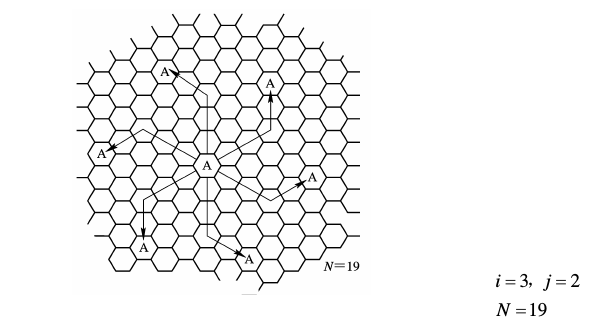
\includegraphics[scale=0.8]{通频道距离确定.png}
		\caption{通频道距离确定}
	\end{figure}
	\begin{minipage}[c]{0.8\linewidth}
			\begin{gather*}
		D^2 = I^2 + J^2 - 2IJ\cos120°	\\
		H = \frac{\sqrt{3}}{2}R	\\
		I = \sqrt{3}iR,J = \sqrt{3}jR	\\
		\Rightarrow 
		D = \sqrt{3N}R,\text{其中}N = i^2+ij+j^2
		\end{gather*} 
	\end{minipage}
	\begin{minipage}[r]{0.2\linewidth}
		\stepcounter{equation}
		(\theequation)
	\end{minipage}
	
	\subsubsection{同频干扰}
	移动台的接收载波干扰比为: \\

	\begin{gather}
		\frac{C}{I} = \frac{C}{\sum_{i=1}^{L}I_i} \notag  \\
		\frac{C}{I} = \frac{(D/R)^n}{L}=\frac{\sqrt{3N}^n}{L} 
		\label{eq:载干比}
	\end{gather}

	其中,L为同频干扰小区数,由于一般是第一层起主要作用,所以L=6(因为采用的是正六边形),则公式可改写为:
	\begin{eqnarray}
	\frac{C}{I} = \frac{(D/R)^n}{L}=\frac{\sqrt{3N}^n}{6} 
	\end{eqnarray}
	n常取4,用Q表示同频复用比例$Q = \frac{D}{R}$。注意:\textbf{\(\frac{C}{I}\)带入计算时要去分贝化}。
	\subsubsection{蜂窝系统容量}
	通常衡量
	系统容量的指标是\textbf{每小区的可用信道数来度量}:
	\begin{equation}
		n = \frac{B_t}{B_cN}
	\end{equation}
	\begin{itemize}
		\item $B_t$ 系统总带宽
		\item $B_c$ 单个小区占用的信道带宽
		\item $N$ 频率复用因子,利用\ref{eq:载干比}载干比来计算
		\begin{equation*}
			N = \sqrt{\frac{2}{3}\times \frac{C}{I}}
		\end{equation*}
	\end{itemize}
		
	\begin{description}
		\item[FDMA系统] 		

		
		\begin{equation}
		n = \frac{B_t}{B_c\sqrt{\frac{2}{3}\times \frac{C}{I}}}
		\end{equation}
		\item [TDMA系统]
		\begin{gather}
			n = \frac{B_t}{B_c^{'}\sqrt{\frac{2}{3}\times \frac{C}{I}}} \notag \\
			B_c^{'} = \frac{B_c}{m}
		\end{gather}
		\begin{itemize}
			\item 	$B_c^{'}$是等效带宽。相当于原来一个频道带宽又分给了多个时隙。
			\item  		m是每一频道包含的时隙数。
		\end{itemize}
		TDMA采用了数字技术,要求的载干比比FDMA的小,N值也比较小。
		\item[CDMA系统] 
		\begin{equation}
		n = [1+\frac{W/R_b}{E_b/I_0}\times \frac{1}{d}]\times G\cdot F
		\end{equation}
		\begin{itemize}
			\item  $E_b/I_0$
			是归一化信噪比,计算时需要\textbf{去分贝化}
			\item $W/R_b$是系统的扩频因子,即系统的处理增益。
			\item d是占空比
			\item G为扇区分区系数
			\item F信道复用系数
		\end{itemize}
	\end{description}
	\subsubsection{几种蜂窝系统的比较}
	\begin{itemize}
		\item FMDA和TDMA是频率受限系统,影响因素:频率与载干比
		\item CMDA是干扰受限系统,影响因素:扩频处理增益,信噪比,占空比,扇区分区系数,信道复用系数等。
	\end{itemize}
	\subsubsection{提高蜂窝系统容量的方法
	}
	\begin{enumerate}
		\item 	基站发射机位置
		\begin{enumerate}
			\item  中心激励小区:安置在小区的中心
			\item  顶点激励小区:安置在六边形3个间隔的顶点上 \\
			\begin{center}
			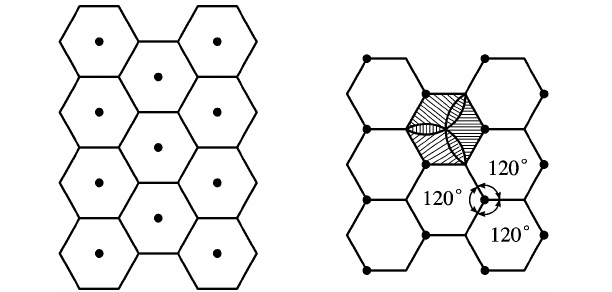
\includegraphics[scale=0.7]{基站发射机位置.png}
			\end{center}
		\end{enumerate}
		\item 小区分裂,\textbf{增加信道的复用次数}。
		\item 划分扇区,\textbf{使用定向天线减少同频干扰}。
		\item 新微小区,在微小区见运动时\textbf{不需要进行越区切换},保证覆盖范围的同时也\textbf{减小了同频干扰}。
	\end{enumerate}
	\subsection{多信道共用技术}
	\begin{itemize}
		\item 信道 --> (1)控制信道CCH,(2)业务信道THH
		\item 信道共用,原因:移动通信的频率资源十分紧缺,一个基站不可能为
		其所覆盖小区的每一个移动台预留一个专用的信道,
		而是采用信道共用的方式。
		\begin{center}
			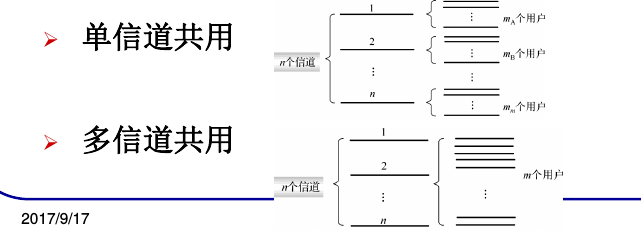
\includegraphics[width=\linewidth,height=4cm]{信道共用.png}
		\end{center}
	\end{itemize}
	\subsubsection{话务量}
	\begin{itemize}
		\item 话音业务量,用话务量描述。
		\begin{itemize}
			\item 流入话务量$A = Ct$,C为单位时间内平均发生的呼叫次数,t为每次呼叫平均占用信道时间。
			\item 完成话务量$A_0=C_0t_0$,$A_0$完成话务量,$C_0$为呼叫成功次数,t伪呼叫平均占用信道时间。
		\end{itemize}
		\item 非话音业务量,用信息流量来描述。
	\end{itemize}
	话务量是通过链路到达交换机的\textbf{总业务量}。现在要求系统能够容纳的系统用户数量,首先求解单个用户所需话务量:
	单个用户忙时话务量:
	\begin{eqnarray}
		\alpha = CTk\frac{1}{3600}
	\end{eqnarray}
	其中,C,T同上,k为集中系数,即忙时话务量对全天话务量之比。
	所以:
	n个共用信道所能容纳的总用户数:
	\begin{eqnarray}
		N = mn = \frac{A}{\alpha}
	\end{eqnarray}
	每个共用信道所能容量的用户数m:
	\begin{eqnarray}
		m = \frac{A/n}{\alpha}
	\end{eqnarray}
	n为共用信道数个数。
	\subsubsection{呼损率和爱尔兰公式}
	流入话务量-完成话务量=损失话务量。\textbf{呼损率B=}损失话务量/流入话务量:
	\begin{eqnarray}
		B = \frac{A-A_0}{A}
	\end{eqnarray}
	损失话务量越低服务质量越高,公网长取0.05,要提高B只有降低A。\\
	话务理论的经典公式-爱尔兰呼损公式:
	\begin{equation}
		B = \frac{A^n/n}{\sum_{i=0}^{n}A^i/i!}
	\end{equation}
	其中,
	\begin{itemize}
		\item B,呼损率
		\item A,流入话务量
		\item n,共用信道数
	\end{itemize}
	 信道利用率公式
	\begin{equation}
	\eta = \frac{A(1-B)}{n}
	\end{equation}


	 \textbf{用途:}\\
	 \begin{itemize}
	 	\item 计算共用信道n。
	 	\item 计算总用户量M。
	 \end{itemize}
	\subsection{网络结构}
	\begin{figure}[H]
		\centering
		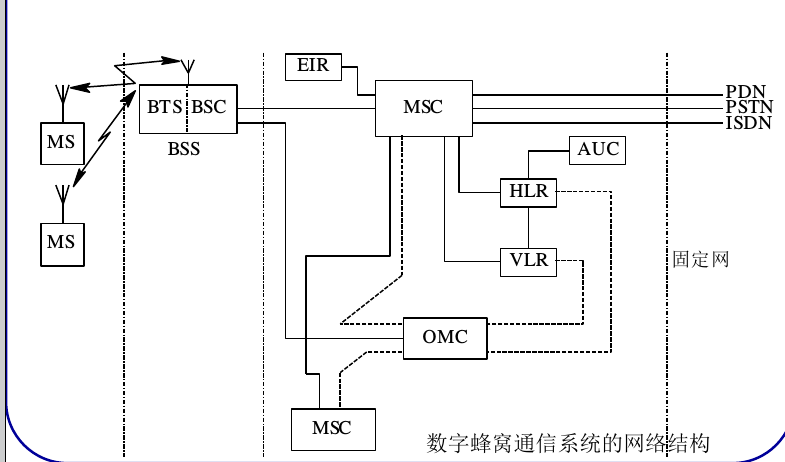
\includegraphics[width=0.8\linewidth]{网络结构.png}
		\caption{网络结构}
	\end{figure}
	\begin{enumerate}
		\item MS--移动台。如:手机,车载终端。
		\item BTS--基站收发信机。处理网络侧的无线信号收发。和MS直接交互。
		\item BSC--基站控制器。一个BSC连接1--255个BTS。
		\item MSC--移动交换中心。MSC与VLR一一对应,工程上又称为MSC/VLR。MSC的主要功能有:
		\begin{enumerate}
			\item 路由管理
			\item 业务量管理:短信,电话,流量。
			\item 计费和费率管理,为用户通信时间生成详细话单记录。
			\item 向HLR发送有关业务量和计费信息。
		\end{enumerate}
		\item VLR--访问位置寄存器,功能:
		\begin{enumerate}
			\item MS漫游号码管理。
			\item TMSI分配与管理。(临时用户移动用户表示,移动台地址)
			\item 用户参数管理
			\item 用户鉴权。
			\item HLR更新。
			\item 管理MSC区、位置(LA)区及基站区。
			\item 无线资源管理。
		\end{enumerate}
		\item HLR--归属位置寄存器。(一个用户只和一个HLR关联,即用户的SIM卡和HLR关联)
		\begin{enumerate}
			\item 管理和维护在HLR中等级注册的所有用户的参数。用户的MSISDN号码(被叫号码,如公司里的短号);;用户定制的业务信息;智能业务(VPN
			组网等);IMSI号码(SIM卡号,唯一)。
			\item 计费管理
			\item VLR更新。
		\end{enumerate}
		\item AuC--鉴权认证中心。管理用户的IMSI、密钥、加解密参数、鉴权参数。
	\end{enumerate}
	\subsection{网络的控制与管理}
	\textbf{移动性管理功能:}移动从一个位置区漫游到另一个位置
	区时,网络中的有关位置寄存器要随之对移动台
	的位置信息进行登记、修改或删除 \\
	\textbf{越区:}移动台在\textbf{通过过程中},MS从一个BTS服务区进入另一个BTS服务区,MS与原BTS之间无线链路转到MS与新BTS之间的无线链路上来。
	\subsubsection{越区切换类型}
	\begin{enumerate}
		\item 硬切换:断开与原BTS的链接,再建立和新BTS的链接。GSM
		\item 软切换:先建立与新BTS的链接,再断开和原BTS的连接。CDMA
		\item 接力切换。TD-SCDMA。
	\end{enumerate}
	\subsubsection{越区切换的判定准则}
	\begin{enumerate}
		\item 相对信号强度准则。
		\item 门限规定的相对信号强度准则。
		\item 具有滞后余量的相对信号强度准则。
		\item 具有门限规定和滞后余量的相对信号强度准则。商业
	\end{enumerate}
	\begin{figure}[H]
		\centering
		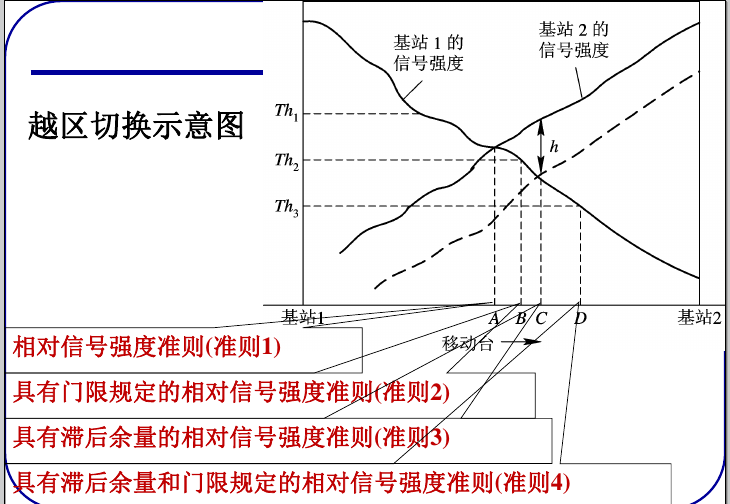
\includegraphics[width=\linewidth]{越区切换判定准则.png}
		\caption{越区切换判定准则}
	\end{figure}
	\subsubsection{越区切换的控制策略
	}
	\begin{enumerate}
		\item 移动控制,测量和判定过程全部由MS完成;
		PHS
		\item 网络控制,测量和判定过程全部由网络完成;
		AMPS
		\item 移动台辅助控制,测量由移动台来完成,判决
		由网络来完成。
	\end{enumerate}
	\subsubsection{越区切换时的信道分配
	}
	为了使得越区失败的概率尽量小,常用
	的做法是在每个小区预留部分信道专门用
	于越区切换。
	\subsubsection{位置管理}
	\begin{enumerate}
		\item \textbf{位置登记:}当用户开关机或者在位置区
		(LAI或REG\_ZONE(CDMA))之间移动或者经
		历了一个固定的时间间隔的时候,移动台需
		要向网络报告它的位置.开机登记、关机登记、基于时间登记、\\
		基于位置区变更登记.
		当一个移动终端(MT)进入一个新的RA时, 位置
		登记过程分为三个步骤:
		\begin{itemize}
			\item  在管理新RA的新VLR中登记MT;
			\item  修改HLR中记录服务该MT的新VLR的ID;
			\item 在旧VLR和MSC中注销该MT。
		\end{itemize}
		\textbf{具体过程:}\\
		\begin{figure}[H]
			\centering
			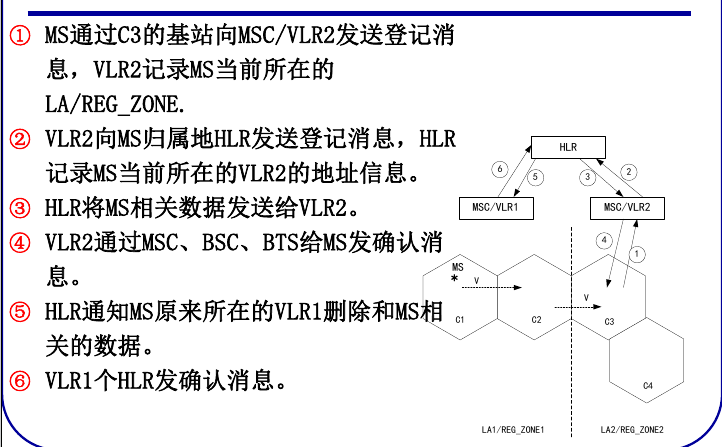
\includegraphics[width=\linewidth]{位置区切换过程.png}
			\caption{位置区切换过程}
		\end{figure}
	\item 呼叫传递:
	\begin{figure}[H]
		\centering
		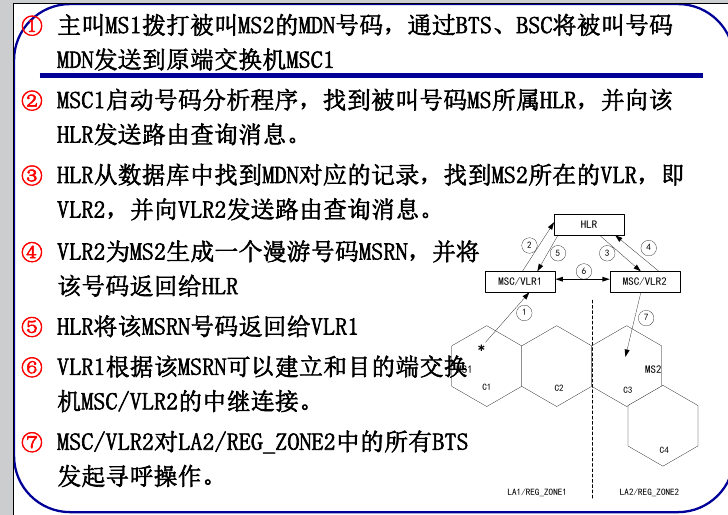
\includegraphics[width=\linewidth]{呼叫传递.png}
		\caption{呼叫传递过程}
	\end{figure}
	\end{enumerate}

=======
	\chapter{概论}
	\section{移动通信特点}
	\subsection{什么是移动通信?}
	\textbf{定义:}移动通信就是通信双方至少有一方是处于运动中进行信息交换的通信方式。其移动性包括:
	\begin{itemize}
		\item 终端的移动性,特定的“终端号码(如手机串号,\verb|*#06#| )“,手机,车载台
		\item 个人的移动性,特定的”个人号码,SIM卡号”。
	\end{itemize}
	\subsection{移动通信特点}
	\begin{enumerate}
		\item 移动通信必须利用无线电波进行信息传输。
		\begin{enumerate}
			\item 弥散损耗(自由传播损耗),随着传播距离的增加而损耗。
			\item 阴影效应,受到地形、地物的遮蔽而发生。
			\item 多径效应,信号经过多点反射,会从多条路径到达接受地点,这种多径信号的\textbf{幅度、相位和到达时间}都不一样,它们会叠加而产生“多径效应”。
			\item 多普勒-效应
		\end{enumerate}
		\item 移动通信是在复杂的干扰环境中运行的。
		\begin{enumerate}
			\item 外部干扰。天电干扰、工业干扰和信道噪声
			
			\item 系统间干扰。
			\begin{enumerate}
				\item 邻道干扰
				\item 互调干扰(当两个或多个干扰信号同时加到接收机时,\textbf{由于非线性的作用},这两个干扰的组合频率有时会恰好等于或接近有用信号频率而顺利通过接收机,这种干扰就称为互调干扰,其中三阶互调最严重。)
				\item 同频道
				干扰(蜂窝移动通信)
				\item 多址干扰(多址干扰是指同\textbf{CDMA}系统中多个用户的信号在时域和频域上是混叠的。因为\textbf{CDMA}系统为码分多址,CDMA系统采用的是不同的地址码来区分每个用户,但多个用户的信号在时域和频域上是混叠的,所以在频域在产生一定的同频和邻频干扰,则为多址干扰。)
				\item 远近效应
			\end{enumerate}
			
			\item 抗干扰技术。扩频技术、信道编码与交织技
			术、信道均衡技术、分集技术、信道估计技
			术、信号检测技术和智能天线技术
			
		\end{enumerate}
		\item 移动通信业务量的需求与日俱增,而频率资源
		非常有限。
		\item 移动通信系统的网络结构多种多样,网络管
		理和控制必须有效。
		\item 移动通信设备必须适于在移动环境中满足多种应
		用要求。
	\end{enumerate}
	\section{常用移动通信系统}
	\begin{enumerate}
		\item  公共陆地移动通信网络(PLMN)
		\item 无线市话系统(WUTS)
		\item 集群系统(专网)--->公安系统,水利系统、交通系统、电力系统、铁路系统。
		\item 卫星移动通信系统。
		\item 无线局域网。
	\end{enumerate}
	\section{移动通信系统发展}
	\begin{figure}[H]
		\centering
		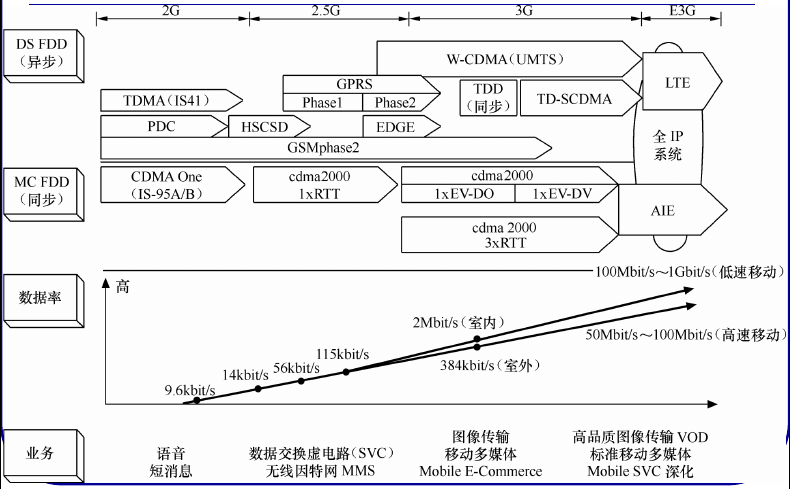
\includegraphics[scale=0.7]{移动通信系统2G_4G发展.png}
		\caption{移动通信系统发展}
	\end{figure}
	\begin{figure}[H]
		\centering
		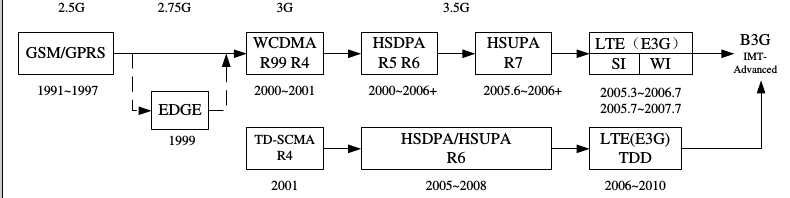
\includegraphics[scale=0.7]{WCDMA_TD-SCDMA发展.png}
		\caption{WCDMA\&TD-SCDMA发展}
	\end{figure}
	\begin{figure}
		\centering
		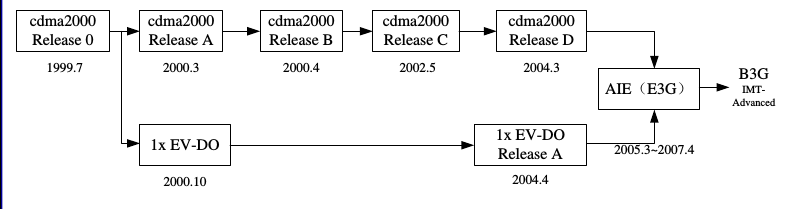
\includegraphics[scale=0.7]{CDMA2000发展.png}
		\caption{CDMA2000发展}
	\end{figure}
	\section{蜂窝移动通信的组网技术}
	\subsection{多址接入}
	\subsubsection{什么是多址接入?}
	\textbf{定义:}移动通信系统中,使所有的用户共享
	有限的无线资源,实现不同用户不同地点同时
	通信,并尽可能减少干扰。
	\subsubsection{多路复用和多址接入区别}
	\textbf{相同点:}两者的理论基础都是\textbf{信号的正交分割原理。}
	
	\textbf{不同点:}
	\begin{itemize}
		\item \textbf{”点对点“},多路复用
		\item \textbf{"点多多点"},多址接入
	\end{itemize}
	
	\subsubsection{多址接入分类}
	\begin{enumerate}
		\item 频分多址: 第一代移动通信系统;TACS、AMPS。
		\item 时分多址: 第二代移动通信系统:GSM。
		\item 码分多址: 第三代移动通信系统:IS-95 CDMA、WCDMA。存在两个重要问题:
		\begin{enumerate}
			\item  多址干扰
			\item  远近效应.
		\end{enumerate}
		\item 空分多址。
		\item OFDMA.正交频分多址
		\item NOMA,非正交频分多址
	\end{enumerate}
	\subsection{工作方式}
	\begin{enumerate}
		\item 单工::通信双方电台交替地进行收信和
		发信。\textbf{对讲机}。
		\item 半双工:是指通信双方中,一方使用双
		频双工方式,即收发信机同时工作;另一
		方使用双频单工方式,即收发信机交替工
		作。\textbf{基站-手机}。基站处于全双工,手机处于半双工。
		\item 全双工:是指通信双方收发信机均同时工
		作。收信和发信必须\textbf{采用不同的工作频率},\textbf{打电话}	\\
		
		双工模式:
		\begin{enumerate}
		\item 频分双工FDD。
		\item 时分双工TDD。
		\end{enumerate}
		两种模式的区别:
		\begin{itemize}
			\item 由于TDD方式的时间资源\textbf{分别分给了上行和下行,
			因此TDD方式的发射时间大约只有FDD的一半},如果
			TDD要发送和FDD同样多的数据,就要\textbf{增大TDD的发
			送功率。}
			\item TDD可以通过调整上下行时隙转换点,改变上下行
			时隙比例,可\textbf{很好地支持非对称业务}。
			\item TDD系统上行受限,因此TDD基站的\textbf{覆盖范围明显小}
			于FDD基站。
			\item FDD模式的特点是在分离(上下行频率间隔45MHz、
			190MHz等)的两个对称频率信道上,系统进行接收
			和传送,用保护频段来分离接收和传送信道。相当
			于分道行驶,比较顺畅,所以\textbf{FDD速度会更快}。
			
		\end{itemize}
%		\hspace{-5em}
		\begin{center}
			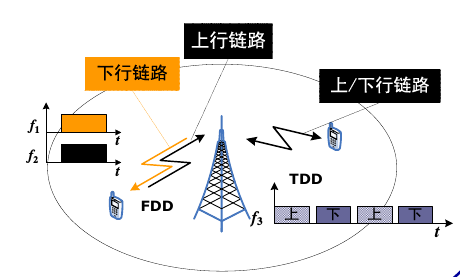
\includegraphics[scale=1]{双工模式.png}
		\end{center}
	\end{enumerate}
	\subsection{频率复用和蜂窝小区}
	\subsubsection{移动通信网的区域覆盖方式}
	\begin{enumerate}
		\item 小容量的大区制(发射功率大)
		\item  大容量的小区制,(频率复用)
	\end{enumerate}
	\subsubsection{区群}
	 \textbf{定义:}共同使用全部可用频率的N个小区组成一个区群。\\
	 \textbf{特点:}
	 \begin{enumerate}
	 	\item 同一个小区,使用不同的频率。
	 	\item 不同小区,可以使用相同频率。
	 \end{enumerate}
 	\textbf{组成区群的小区数对应的公式}:
 	\begin{eqnarray}
 		N = i^2+ij+j^2
 	\end{eqnarray}
	一个共有S个信道的蜂窝系统(一个区群),每簇含有N个小区(一个区群),每个小区含有K个信道。则:
	\begin{eqnarray}
		S = KN
	\end{eqnarray}
	将这个簇重复M次,则信道总数为C:
	\begin{eqnarray}
	C = MS = MKN
	\end{eqnarray}
	\subsubsection{同频道距离}
	\textbf{STEPS:}
	\begin{enumerate}
		\item 首先垂直六边形的任一边延长$Max{i,j}$个小区。
		\item 逆时针旋转60°,在延长$Min{i,j}$个小区。
	\end{enumerate}

	\begin{figure}[H]
		\centering
		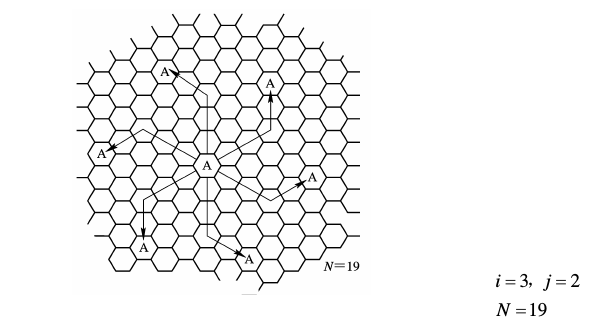
\includegraphics[scale=0.65]{通频道距离确定.png}
		\caption{通频道距离确定}
	\end{figure}
	\begin{minipage}[c]{0.8\linewidth}
			\begin{gather*}
		D^2 = I^2 + J^2 - 2IJ\cos120°	\\
		H = \frac{\sqrt{3}}{2}R	\\
		I = \sqrt{3}iR,J = \sqrt{3}jR	\\
		\Rightarrow 
		D = \sqrt{3N}R,\text{其中}N = i^2+ij+j^2
		\end{gather*} 
	\end{minipage}
	\begin{minipage}[r]{0.2\linewidth}
		\stepcounter{equation}
		(\theequation)
	\end{minipage}
	
	\subsubsection{同频干扰}
	移动台的接收载波干扰比为: \\

	\begin{gather}
		\frac{C}{I} = \frac{C}{\sum_{i=1}^{L}I_i} \notag  \\
		\frac{C}{I} = \frac{(D/R)^n}{L}=\frac{\sqrt{3N}^n}{L} 
		\label{eq:载干比}
	\end{gather}

	\text{其中,L为同频干扰小区数} \\
	n常取4,用Q表示同频复用比例$Q = \frac{D}{R}$。
	\subsubsection{蜂窝系统容量}
	通常衡量
	系统容量的指标是每小区的可用信道数来度量:
	\begin{equation}
		n = \frac{B_t}{B_cN}
	\end{equation}
	\begin{itemize}
		\item $B_t$ 系统总带宽
		\item $B_c$ 单个小区占用的信道带宽
		\item $N$ 频率复用因子,利用\ref{eq:载干比}计算
	\end{itemize}
	\begin{description}
		\item[FDMA系统] 
		
		\begin{equation*}
			N = \sqrt{\frac{2}{3}\times \frac{C}{I}}
		\end{equation*}
		
		\begin{equation}
		n = \frac{B_t}{B_c\sqrt{\frac{2}{3}\times \frac{C}{I}}}
		\end{equation}
		\item [TDMA系统]
		\begin{gather}
			n = \frac{B_t}{B_c^{'}\sqrt{\frac{2}{3}\times \frac{C}{I}}} \notag \\
			B_c^{'} = \frac{B_c}{m}
		\end{gather}
		m是每一频道包含的时隙数。
		\item[CDMA系统] 
		\begin{equation}
		n = [1+\frac{W/R_b}{E_b/I_0}\times \frac{1}{d}]\times G F
		\end{equation}
	\end{description}
	\subsubsection{提高蜂窝系统容量的方法
	}
	\begin{enumerate}
		\item 	基站发射机位置
		\begin{enumerate}
			\item  中心激励小区:安置在小区的中心
			\item  顶点激励小区:安置在六边形3个间隔的顶点上 \\
			\begin{center}
			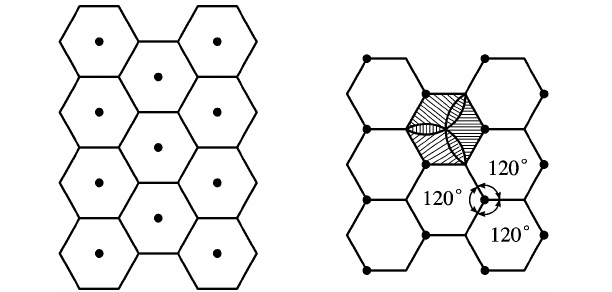
\includegraphics[scale=0.7]{基站发射机位置.png}
			\end{center}
		\end{enumerate}
		\item 小区分裂
		\item 划分扇区
		\item 新微小区
	\end{enumerate}
	\subsection{多信道共用技术}
	\begin{itemize}
		\item 信道 --> (1)控制信道,业务信道
		\item 信道共用
		\begin{center}
			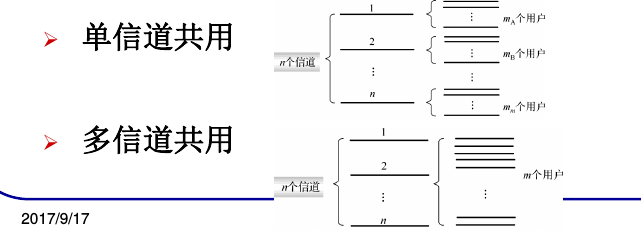
\includegraphics[width=\linewidth,height=4cm]{信道共用.png}
		\end{center}
	\end{itemize}
	话务理论的经典公式-爱尔兰呼损公式:
	\begin{equation}
	B = \frac{A^n/n}{\sum_{i=0}^{n}A^i/i!}
	\end{equation}
	其中
	\begin{itemize}
		\item B,呼损率
		\item A,流入话务量
		\item n,共用信道数
	\end{itemize}
	 信道利用率公式
	\begin{equation}
	\eta = \frac{A(1-B)}{n}
	\end{equation}
	用户忙时话务量:$\alpha = CTk\frac{1}{3600}$ \\
	每个共用信道所能容量的用户数:$m = \frac{A/n}{\alpha}$ \\
	n个共用信道所能容纳的总用户数:$N = mn = \frac{A}{\alpha}$
>>>>>>> master
\end{document}